Pour créer ce logiciel, nous avons utilisé le langage Python. La raison première de ce choix est l'utilisation de Keras et Tensorflow, des bibliothèques de deeplearning. 

\subsection{Une décomposition modulaire du code}

Grâce à une programmation orientée objet, nous avons pu concevoir le logiciel de telle sorte à ce qu'il y ai plusieurs modules interchangeables. Nous avons ainsi trois modules principaux : le moteur, le lanceur et les joueurs. Le moteur permet d'exécuter plusieurs parties de blackjack. Le lanceur permet de configurer le moteur selon les désirs de l'utilisateur et de le démarrer, c'est le point d'entrée du programme. Les joueurs fournissent des implémentations différentes pour chaque algorithme.

Nous avons créé le moteur de telle sorte qu'il soit totalement hermétique à l'implémentation d'un joueur et de la manière dont le moteur est utilisé. De plus, nous avons rendu le moteur très configurable dans son exécution. C'est-à-dire que le moteur seulement n'est pas capable de lancer des parties de blackjack et d'y jouer. Nous avons conçu le moteur comme une bibliothèque qui a besoin d'un code client pour exploiter tout son potentiel. C'est celui-ci qui viendra définir les paramètres d'exécution ainsi que les différentes implémentations de joueurs.
En effet, le moteur se base sur l'abstraction d'un joueur. Cette abstraction nous a permis plus tard de pouvoir réaliser différents joueurs qui ont chacun un algorithme différent sans changer le code du moteur. Nous nous sommes servis de la programmation objet et du principe de substitution de Liskov ainsi que de l'inversion de dépendances pour faire cela.

Le lanceur est le module qui sert d'entrée du programme. C'est celui-ci qui va paramétrer le moteur, lui fournir les joueurs et lancer la partie. Le lanceur que nous avons fait est en ligne de commande et utilise les arguments définis par l'utilisateur pour paramétrer le moteur.

Le module joueur fourni les différentes implémentations de joueur. Nous avons créé un joueur par algorithme. Les algorithmes étant "Basique", "Hi-Lo", "Hi-Lo No Count", "Deep Learning" et humain (bien qu'il n'y ai pas réellement d'algorithme).

Nous avons un quatrième module pour gérer l'affichage des données et du jeu. De même que pour les joueurs, le moteur se sert d'une abstraction de l'affichage pour permettre d'avoir plusieurs types d'affichages possibles sans modification du code du moteur. Nous avons créé une implémentation de l'affichage qui est en mode textuel dans un terminal.

\subsection{Diagramme de classes}

La page ci-dessous présente le diagramme de classes simplifié représentant les interactions entre les classes de l'application. Celui-ci ne contient pas les attributs et méthodes des différentes classes. C'est pourquoi, une \hyperref[subsec:class-diagram]{version complète du diagramme de classe}  se trouve en annexe.

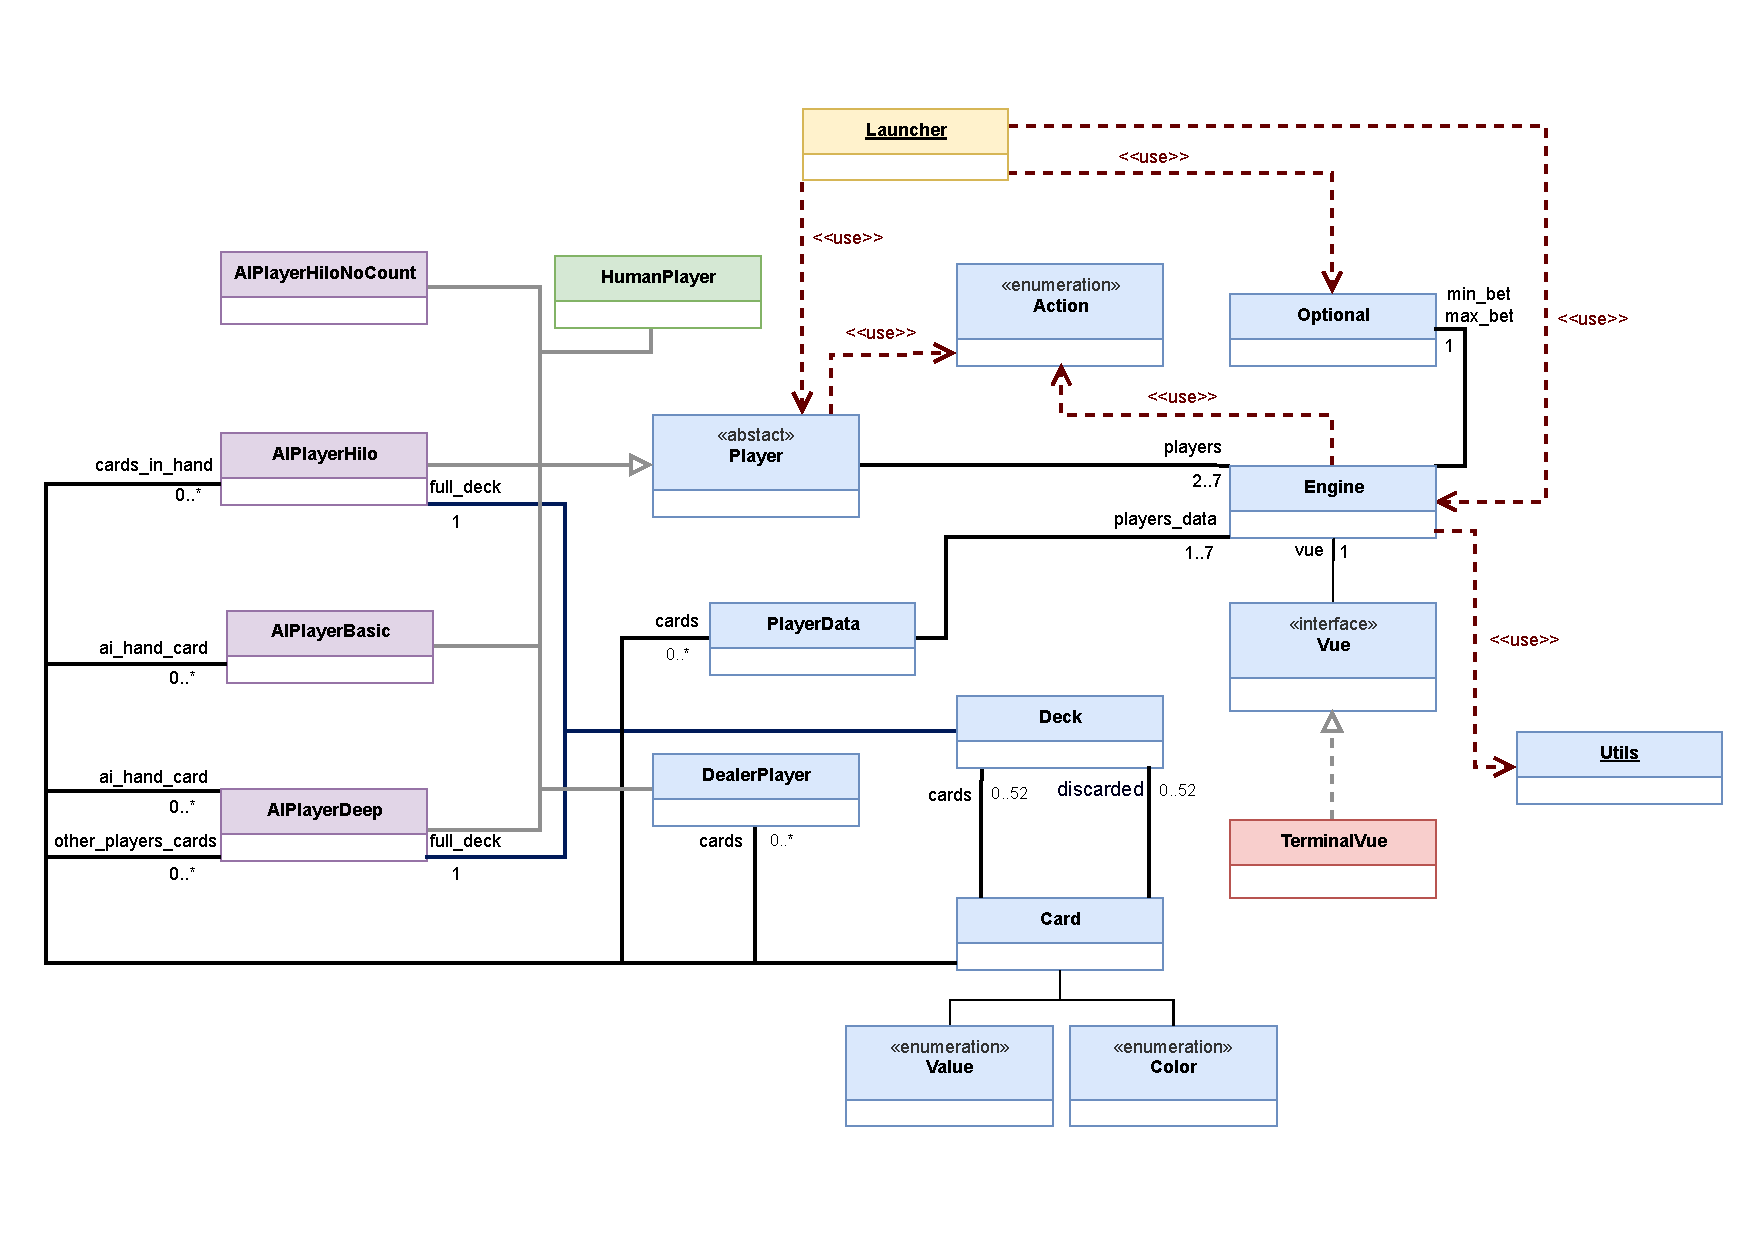
\includepdf[landscape=true]{3-architecture/simplified_class_diagram.pdf}

\begin{figure}[H]
\caption{Diagramme de classes simplifié représentant les interactions entre les classes de l'application}
\label{fig:simplified_class_diagram}
\end{figure}

\subsection{Bibliothèques externes utilisées}

Pour développer l'implémentation d'un joueur se basant sur le deeplearning, nous nous sommes servis des bibliothèques TensorFlow \cite{ref-tensorflow}, Keras \cite{ref-keras}, NumPy \cite{ref-numpy} et Pandas\cite{ref-pandas}. TensorFlow et Keras sont des bibliothèques permettant de faire des calculs de deeplearning. NumPy sert à faire des calculs mathématiques et est utilisée par TensorFlow. Pandas sert à manipuler facilement les données d'un fichier CSV. Sans ces bibliothèques, il nous aurait été impossible de produire une IA basée sur du deeplearning.

De plus, nous avons utilisé deux fonctions utilitaires dans le moteur que nous avons trouvé sur StackOverflow. Le lien vers la page est renseigné au niveau de la documentation du code.

\subsection{Implémentation du jeu}

Pour implémenter l'exécution d'une partie de jeu et faire en sorte que les joueurs aient toutes les données du plateau de jeu à chaque instant, nous avons mis en place plusieurs évènements afin de donner aux joueurs les nouvelles informations.

Il y a deux évènements, le début de la partie et sa fin, qui sont obligatoires et lancés à chaque partie. Il est assuré qu'ils ne sont lancés qu'une seule fois par partie.

Les autres évènements sont optionnels et multiples. C'est-à-dire qu'un de ceux-ci peut ne pas être lancé durant une partie, comme il peut être lancé plusieurs fois. Ces évènements sont "gain d'une nouvelle carte", "un autre joueur a gagné une carte", "le croupier a gagné une carte", et "la défausse a été remise dans la pioche".

Ainsi, au début de la partie, le moteur va notifier les joueurs du début de la partie, puis demander leur mise. Une fois les mises définies, le moteur notifie les joueurs de leurs cartes, de celles de leurs camarades et celle visible du croupier. Ensuite, pour chaque joueur le moteur demande les actions que le joueur décide de faire et notifie les joueurs du résultat de l'action. Une fois que chaque joueur a terminé toutes ses actions, le moteur notifie le joueur des cartes piochées par le croupier puis les notifie de la fin de la partie.

\begin{figure}[H]
    \begin{tikzpicture}
    \begin{umlseqdiag}
        \umlobject{Engine}
        \umlobject{Player1}
        \umlobject{Player2}
        \begin{umlcall}[op={notify\_game\_start()}]{Engine}{Player1}
        \begin{umlcall}[op={notify\_game\_start()}]{Engine}{Player2}
        \begin{umlcall}[op={get\_bet()}, return=value]{Engine}{Player1}
        \end{umlcall}
        \begin{umlcall}[op={get\_bet()}, return=value]{Engine}{Player2}
        \end{umlcall}
        \begin{umlcall}[op={notify\_new\_card()}]{Engine}{Player1}
        \end{umlcall}
        \begin{umlcall}[op={notify\_new\_bud\_card()}]{Engine}{Player2}
        \end{umlcall}
        \begin{umlcall}[op={notify\_new\_card()}]{Engine}{Player2}
        \end{umlcall}
        \begin{umlcall}[op={notify\_new\_bud\_card()}]{Engine}{Player1}
        \end{umlcall}
        \begin{umlcall}[op={notify\_new\_dealer\_card()}]{Engine}{Player1}
        \end{umlcall}
        \begin{umlcall}[op={notify\_new\_dealer\_card()}]{Engine}{Player2}
        \end{umlcall}
        \begin{umlcall}[op={notify\_new\_card()}]{Engine}{Player1}
        \end{umlcall}
        \begin{umlcall}[op={notify\_new\_bud\_card()}]{Engine}{Player2}
        \end{umlcall}
        \begin{umlcall}[op={notify\_new\_card()}]{Engine}{Player2}
        \end{umlcall}
        \begin{umlcall}[op={notify\_new\_bud\_card()}]{Engine}{Player1}
        \end{umlcall}
        \begin{umlfragment}[type=loop, name=play1]
            \begin{umlcall}[op={next\_action()}, return=action]{Engine}{Player1}
            \end{umlcall}
        \end{umlfragment}
        \umlnote[x=-4, y=-12]{play1}{tant que Player1 peut jouer}
        \begin{umlfragment}[type=loop, name=play2]
            \begin{umlcall}[op={next\_action()}, return=action]{Engine}{Player2}
            \end{umlcall}
        \end{umlfragment}
        \umlnote[x=-4, y=-14]{play2}{tant que Player2 peut jouer}
        \begin{umlcall}[op={notify\_game\_end()}]{Engine}{Player1}
        \end{umlcall}
        \begin{umlcall}[op={notify\_game\_end()}]{Engine}{Player2}
        \end{umlcall}
        \end{umlcall}
        \end{umlcall}
    \end{umlseqdiag}
    \end{tikzpicture}
    \caption{Diagramme de séquence décrivant le déroulement simplifié d'une partie.}
\end{figure}
